\documentclass[landscape,footrule]{foils}
\usepackage[lecture-serie]{foiltex-extra}
\usepackage{crysymb}
\usepackage{graphics}
\usepackage[pdftex]{graphicx} 
\usepackage[dvipsnames]{xcolor}
\usepackage{soul}



\newcommand{\lecture}{Frequentist methods}
\newcommand{\lserie}{LTAT.02.004 Machine Learning II}
\newcommand{\ldate}{February 24, 2025}
\newcommand{\lauthor}{Sven Laur}
\newcommand{\linst}{University of Tartu}
\graphicspath{{./illustrations/}}


\newcommand{\leqm}{\ \leq_m}


\newcommand{\bigvskip}{\vskip 2em}
\newcommand{\lastline}{\vspace*{-2ex}}
\newcommand{\spreadappart}{\vspace*{\fill}}

\DeclareMathOperator{\supp}{supp}
\DeclareMathOperator{\conf}{conf}
\DeclareMathOperator{\precision}{precision}
\DeclareMathOperator{\recall}{recall}
\renewcommand{\vec}[1]{\boldsymbol{#1}}


\begin{document}
\titlefoil

\foilhead[-1cm]{Why does empirical risk converge at all?}
\enlargethispage{1cm}
\centerline{
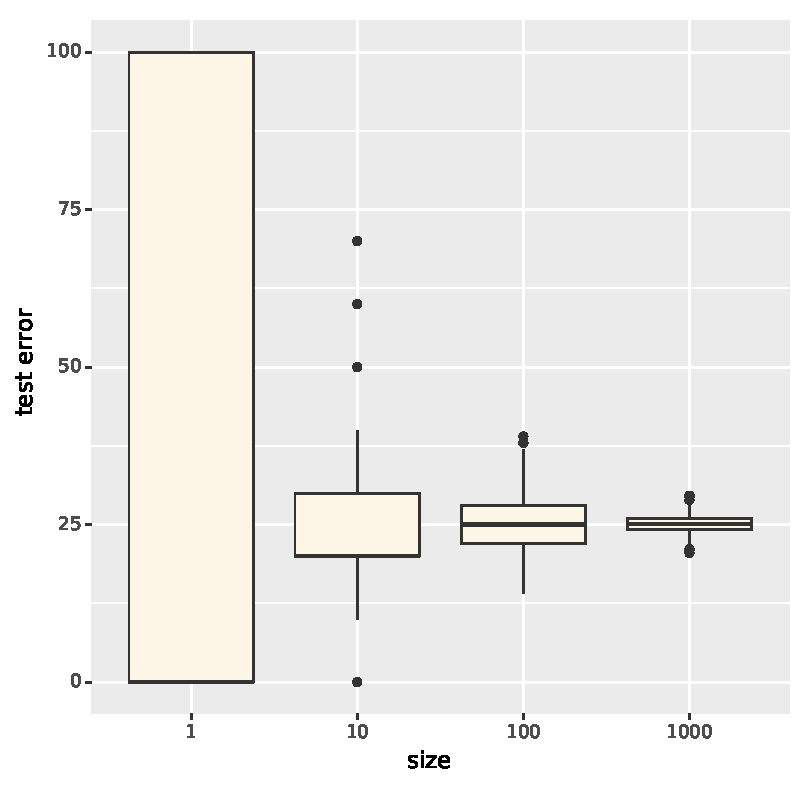
\includegraphics[scale=0.8]{test_error_fluctuations_1}\hspace*{0.5cm}
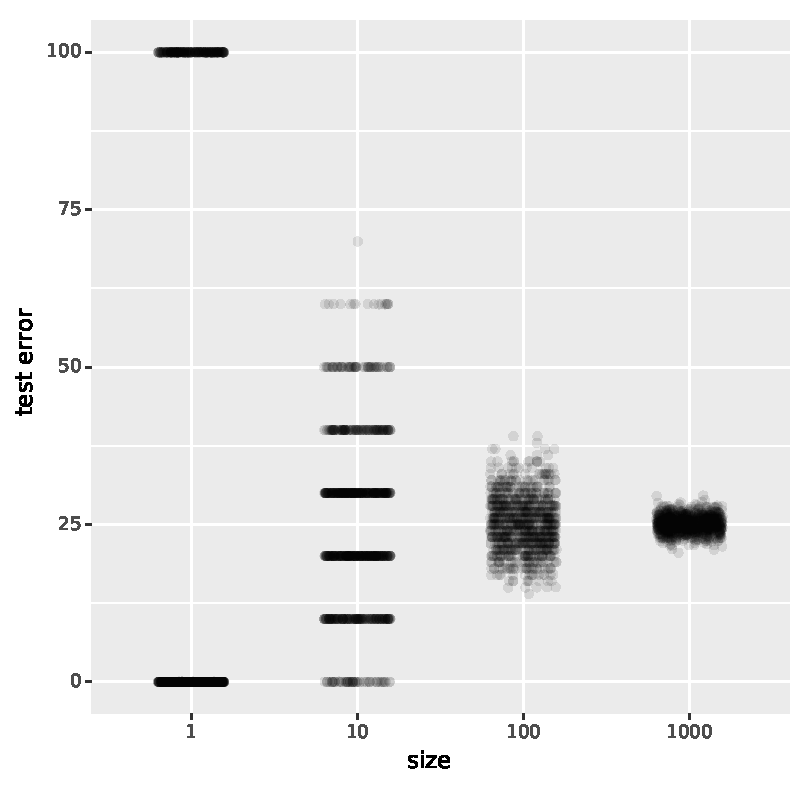
\includegraphics[scale=0.8]{test_error_fluctuations_2}}

\vspace*{-0.0cm}
$\triangleright$  Depends on the test set.\\
$\triangleright$  Statistical fluctuations decrease with size.


\foilhead[-1cm]{Empirical risk as mean of random variables}

\illustration[height=4cm]{single-loss-term}

Recall that empirical risk is computed through the following formula
\begin{align*}
  R_N(f)=\frac{1}{N}\cdot\sum_{i=1}^N L(f(\vec{x}_i), y_i) = \frac{1}{N}\cdot\sum_{i=1}^N z_i
\end{align*} 
where all samples $(\vec{x}_i, y_i)$ are assumed to be
\begin{triangles}
\item independent from each other,
\item coming from the same distribution.
\end{triangles}

\foilhead[-1cm]{Law of large numbers}

\textbf{Central limit theorem.}
Let $z_1, \ldots, z_N$ be independent and identically distributed samples form a \emph{real-valued distribution} with a \emph{finite standard deviation} $\sigma$ and \emph{mean} $\mu$. Then the random variable 
\begin{align*}
S=\sqrt{N}\Biggl(\frac{1}{N}\cdot \sum_{i=1}^N z_i -\mu\Biggr)
\end{align*}
converges \emph{in distribution} to normal distribution $\NNN(mean=0, sd=\sigma)$.  
\vspace{1ex}

\begin{triangles}
\item Under mild assumptions the empirical risk $R_N(f)$ converges to risk $R(f)$.
\item The result is not precise enough to quantify approximation error.
\end{triangles}



\foilhead[-0cm]{What is probability?}

\begin{center}
\includegraphics[height = 5cm]{electron-difraction}\hspace*{0.5cm}
\includegraphics[height = 5cm]{lightning}\hspace*{0.5cm}
\includegraphics[height = 5cm]{coin-flip}
\end{center}
\vspace*{1cm}

Probability is a measure of uncertainty which can rise in several ways
\begin{triangles}
\item Intrinsic uncertainty in the system 
\item Uncertainty caused by inherent instability of the system
\item Uncertainty caused by lack of knowledge or control over the system
\end{triangles}

\foilhead[-1cm]{Frequentistic interpretation of  probability}

\illustration[height=8cm]{rolling-dice}


Probability is an average occurrence rate in long series of experiments.

\begin{triangles}
\item Law of large numbers
\item Probability is a collective property 
\item Probabilities can be assigned only to future events
\end{triangles}



\foilhead[-1cm]{Bayesian interpretation of probability}


\illustration[height=8cm]{shell-game}
Probability reflects persons individual beliefs on future or unknown events. 

\begin{triangles}
\item Belief updates through the Bayes rule
\item Probability is an inherently subjective property 
\item Probabilities can be assigned  to past, present and future events
\end{triangles}



\foilhead[-1cm]{Ultra-frequentistic interpretation of probability}

\illustration[height=8cm]{pigsfly}

Events with small enough probability do not occur
\begin{triangles}
\item The main tool in classical statistics 
\item Errors in judgement does not matter if a gamma ray pulse kills us.
\item One must avoid the lottery paradox in the reasoning
\end{triangles}


\foilhead[-1cm]{The goal of statistical inference}

\textbf{Frequentist goal}
\begin{triangles}
\item The aim of statistics is to design algorithms that work well on average.
\item For that one needs to specify probabilistic model for data sources.
\item Confidence is the fraction of cases the algorithm works as specified.
\end{triangles}
\vspace*{2cm}

\textbf{Bayesian goal}
\begin{triangles}
\item The aim of statistics is to design algorithms that allow \emph{rational individuals} to reliably update their beliefs through Bayes formula.
\item Besides the data source model one has to provide model for initial beliefs.
\item Correctness of an algorithm does not make sense.
\end{triangles}

\middlefoil{Frequentistic methods}

\foilhead[-1cm]{Illustrative example}

Consider an experiment that yields 2 heads and 8 tails.
\begin{triangles}
\item Frequency of heads is $20\%$.
\item Can the coin be still fair?
\end{triangles}
\vspace*{1cm}
 
Consider an experiment that yields 1,000,100 heads and 999,900 tails.
\begin{triangles}
\item Frequency of heads is $50.005\%$.
\item Can the coin be still biased?
\end{triangles}


\foilhead[-1cm]{Central question in statistical testing}

\vspace*{1ex}
\illustration[scale=1.1, trim=3cm 18cm 3cm 3cm, clip]{effect_signifficance_tradeoff}
\vspace*{-2ex}
The question is my observation relevant has two aspects
\begin{triangles}
\item Can we explain the difference by sheer luck? 
\item Is the difference between expected and observed big enough?
\end{triangles}

\foilhead[-1cm]{Causation between zero-one events}

Assume that condition A causes the event $B=1$ with probability $p$, i.e.,
\begin{align*}
\pr{B=1|A}=p
\end{align*}
Then the probability is to get $k$ ones in $n$ independent trials is
\begin{align*}
\pr{B_1+\cdots+B_n=k|A}=\binom{n}{k}p^k(1-p)^{n-k}
\end{align*} 
The number of ones in known to have a \emph{binomial distribution}
\begin{align*}
 B_1+\cdots+B_n\sim\mathsf{Bin}(n, p)
\end{align*}

\foilhead[-1cm]{Illustration}

\illustration[width=22cm]{binomial_distribution}
\vspace*{-1cm}

The distribution of  $B_1+\ldots+B_n$ depends solely on the number of trials $n$ and the probability $p$. Some values of $B_1+\ldots+B_n$ are very unlikely.

\foilhead[-1cm]{Does a classifier beat a random guess?}

\illustration[width=10cm]{binomial_distribution}

Consider three algorithms on twenty element test set:
\begin{diamonds}
\item Algorithm A gets 9 correct answers;
\item Algorithm B gets 13 correct answers;
\item Algorithm C gets 17 correct answers.
\end{diamonds}
\vspace*{3ex}
\begin{triangles}
\item Which of them are better than random classifiers?
\item Which of them are classifiers good enough for practical applications?
\end{triangles}


\foilhead[-1cm]{How to build a statistical test}

\textbf{I. Null hypothesis:}
\begin{triangles}
\item The probability of heads in a coinflip is $\pr{B_i=1}=p$.
\end{triangles}
\vspace*{1cm}

\textbf{II. Choose value to compute aka test statistic:} 
\begin{triangles}
\item Our test statistic will be $B_1+\ldots+B_n$.
\end{triangles}
\vspace*{1cm}


\textbf{III. Consequences on the observations:} 
\begin{triangles}
\item The observed sum $B_1+\ldots+B_n\sim\mathsf{Bin}(n=20, p=0.5)$.
\item Limit on the tail probability $\pr{|B_1+\ldots+B_n-10|\geq 6}\leq 5\%$
\end{triangles}
\vspace*{1cm}

\textbf{IV. Test procedure}
\begin{triangles}
\item Reject null hypotesis at \emph{significance level} $5\%$ if $|B_1+\ldots+B_n-10|\geq 6$.  
\end{triangles}
 
 
\foilhead[-1cm]{Properties of statistical tests}

Statistical test is a classification algorithm designed to distinguish a fixed distribution of negative examples specified by a null hypothesis.
\vspace*{2ex}

Any \emph{fixed} classification \emph{rule} can be converted to a statistical test by finding out the percentage of false positives aka \emph{p-value}:
\begin{triangles}
\item There might exists a closed form solution.
\item We can always estimate p-values using simulations. 
\item Observations must be compressed into a single decision value.
\end{triangles}
\vspace*{2ex}

Testing several hypothesis in parallel increases the number of false positives.  
Several p-value adjustment methods are used to correct the issue:
\begin{triangles}
\item Bonferroni correction is almost optimal 
\item FDR correction controls the expected number false positives  
\end{triangles}  
 

\foilhead[-1cm]{Bonferroni correction for tests}

Assume that data is generated so that null hypotheses $\HHH_1,\ldots, \HHH_n$ hold.
\begin{triangles}
\item Then we can still reject some the tests due to bad luck.
\item We can use really naive enough bound visualised below. 
\end{triangles}  

\vspace*{3ex}
\illustration[scale=1.1, trim=3cm 18cm 4cm 3cm, clip]{union_bound}
\vspace*{-2ex}

\foilhead[-1cm]{How far is the true risk?}

\illustration[scale=0.8]{test_error_fluctuations_2}

\begin{triangles}
\item How wide error bars cover true risk for \emph{all} observations? 
\item How wide error bars  cover true risk for \emph{most} observations? 
\end{triangles}


\foilhead[-1cm]{How to build confidence intervals}
 
\textbf{I. Construct a family of statistical tests:}
\begin{triangles}
\item Define a statistical test $T_p$ for all possible parameter values $p$.
\item All tests should share the same test statistic.
\end{triangles}
\vspace*{1cm}

\textbf{II. Perform multiple hypotesis testing for all parameter values:}
\begin{triangles}
\item Accept all parameters values for which p-value is greater than $1-\alpha$.  
\item Output a minimal interval that covers all accepted parameter values.
\end{triangles}
\vspace*{1cm}

\textbf{Rationale}
\begin{triangles}
\item The true parameter value is rejected on $\alpha$-fraction of~possible~observations.
\item For the remaining cases the true value is inside the predicted interval. 
\end{triangles}


\foilhead[-1cm]{Illustration}
\enlargethispage{0.5cm}
\centerline{
\includegraphics[scale=0.8]{bin_conf_intervals_i}
\includegraphics[scale=0.8]{bin_conf_intervals_ii}}
\begin{triangles}
\item Acceptance ranges for different parameter values on the left.
\item Extended parameter ranges covering all accepted parameters on the right.
\item These ranges are the desired confidence intervals.
\end{triangles}


\foilhead[-1cm]{Interpretation of confidence intervals}

\textbf{Definition.}
Confidence interval for a parameter $p$ is an outcome of an approximation algorithm. The algorithm  must output an interval $[\hat{p}-\varepsilon,\hat{p}+\varepsilon]$ such that the true estimate is in the range on $\alpha$-fraction of cases.
\vspace*{2ex}

\textbf{Paradoxical inapplicability}

The definition does not state that the probability $p\in[\hat{p}-\varepsilon,\hat{p}+\varepsilon]$ is $\alpha$!
\begin{triangles}
\item The statement $p\in[\hat{p}-\varepsilon,\hat{p}+\varepsilon]$ is either true or false.
\item There is no probability left. We just \emph{do not know} the answer!
\end{triangles} 
\vspace*{3ex}

\textbf{Ultra-frequentistic resolution}
\begin{triangles}
\item  If $1-\alpha$ is small enough say $5\%$ then the algorithm is always correct. 
\end{triangles}


\foilhead[-1cm]{Illustrative example}

\illustration[scale=0.8]{confidence_intervals_example}

By increasing the length of the interval we increase the fraction of runs for which the true value of $p$ lies in the interval.


\foilhead[-1cm]{Problems with confidence intervals}

\textbf{Inability to capture background knowledge}
\begin{triangles}
\item What if I know that $p\in[0.1,0.2]$ and observe $B_1=\ldots=B_N=1$?
\item Then the estimate $[\hat{p}-\varepsilon,\hat{p}+\varepsilon]$  is clearly wrong although on average this confidence interval is reasonable.
\end{triangles}
\vspace*{2cm}


\textbf{Multiple hypothesis testing}

\begin{triangles}
\item Using several confidence intervals in parallel increases the fraction of cases where some true estimate is out of the predicted range.
\item We can use p-value adjustment methods are used to correct the issue.
\end{triangles}  




\foilhead[-1cm]{Prediction intervals}

Even if we know the true relation $y=f(\vec{x})$ we cannot predict the observation $y_{i}=f(\vec{x}_i)+\varepsilon_i$, as the noise term $\varepsilon_{i}$ is not known ahead.
\begin{triangles}
\item We cannot give upper and lower bounds for $y_i$ which always hold.
\end{triangles}
\vspace*{4ex}

Instead, we can specify a prediction interval $[y_*-\varepsilon, y_*+\varepsilon]$ so that with probability $95\%$ the resulting measurement $y_i$ is in the range.
\begin{triangles}
\item Usually, the analysis is similar to confidence interval derivation.
\end{triangles}  
\vspace*{4ex}

Interpretation of prediction intervals is different from confidence intervals.

\begin{triangles}
\item The probability estimate holds for the particular interval.
\end{triangles}  

\foilhead[-1cm]{Illustrative example}

\illustration{prediction-intervals-example}

By increasing the length of the prediction interval we increase the fraction of future measurements which fall into interval.


\foilhead[-0cm]{Fluctuations in performance profiles}

\centerline{
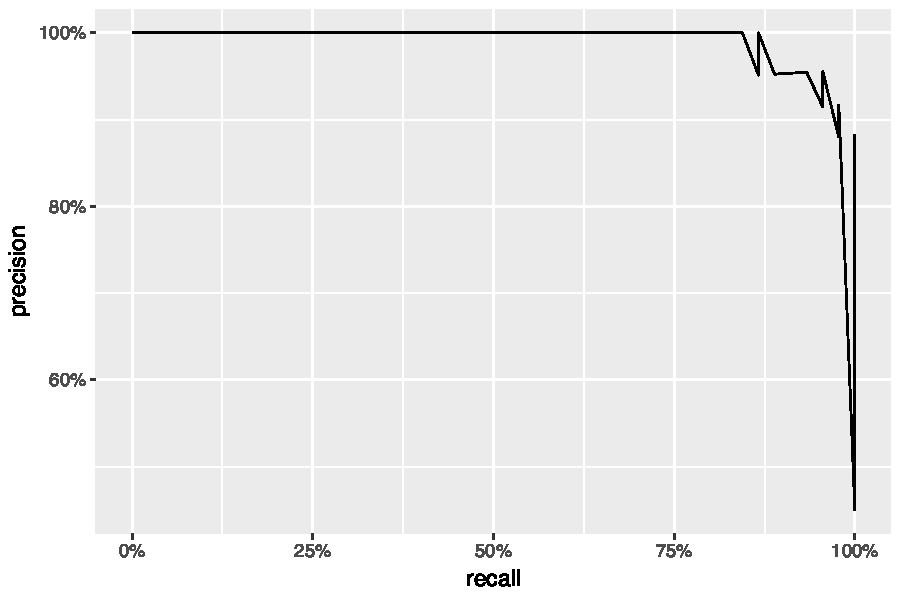
\includegraphics[scale=0.7]{precision_recall_1B}\hspace*{0.5cm}
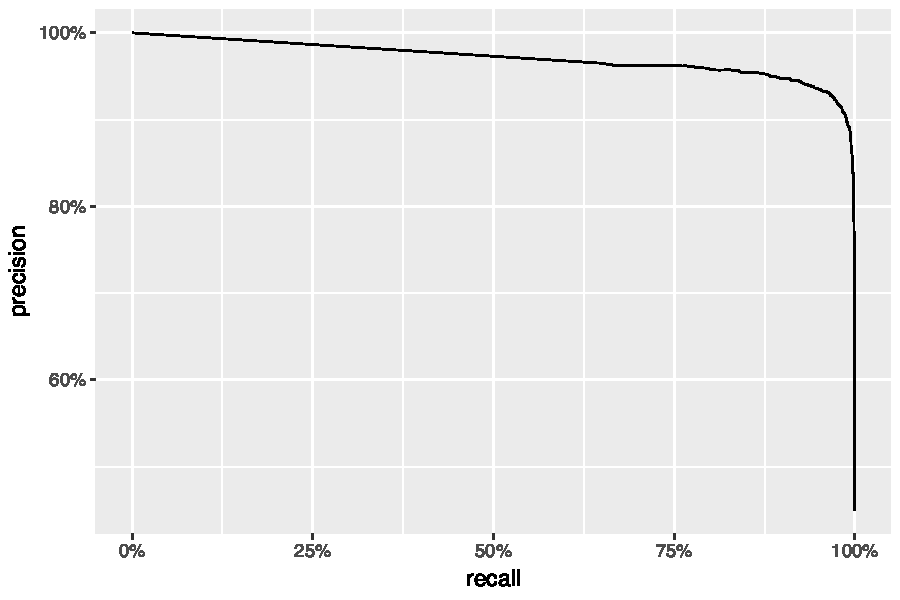
\includegraphics[scale=0.7]{precision_recall_1A}}
\vspace*{1cm}
\begin{triangles}
\item Precision-recall graph is not smooth if the test set is small.
\item How much the true graph can be different from observed?
\item How many of samples are needed to get a decent resolution?  
\end{triangles}


\foilhead[-1cm]{Confidence envelopes}

Confidence intervals is a good way to visualise uncertainty of a particular parameter.
However, we are sometimes interested in the uncertainty many parameters or in the uncertainty of a function:
\begin{triangles}
\item How a predictor $f:[0,1]\to\mathbb{R}$ depends on the training set
\item How a ROC curve $\textsc{Roc}:[0,1]\to[0,1]$ depends on the test set
\item How should a quantile-quantile plot be distributed.
\end{triangles}
\vspace*{4ex}

Confidence bands are generalisations of confidence intervals
\begin{triangles}
\item Pointwise confidence band is a collection of confidence intervals
\item Simultaneous confidence band must enclose $\alpha$-fraction of functions.  
\item Simultaneous confidence bands are much wider than pointwise bands.  
\end{triangles}


\foilhead[-1cm]{Illustrative example}
\enlargethispage{0.5cm}
\centerline{
\includegraphics[scale=0.8]{qq_line_distribution}
\includegraphics[scale=0.8]{qq_confidence_envelope}}
\begin{triangles}
\item Distribution of qq-lines visualised through a sample on the left.
\item A simulation based pointwise $95\%$ confidence envelope on the right.
\item The significance level that qq-line is inside the envelope is ca $50\%$.
\end{triangles}

\foilhead[-1cm]{Permutation tests}

\textbf{Baseline problem:}
\begin{triangles}
\item Achievable accuracy depends on the data distribution. 
\item Artefacts in the dataset may bias performance measures.
\end{triangles}
\vspace*{2ex}

\textbf{Label permutation.}
A random permutation $\pi$ on outputs $y_i$ destroys correlations between input-output pairs $(\vec{x}_{i}, \vec{y}_{\pi(i)})$ but preserves marginal distribution of inputs and outputs. 
\vspace*{2ex}


\textbf{Permutation test.}
Estimate how probable is to achieve equal or higher accuracy than was observed on the real data.
\begin{triangles}
\item If this probability is small then there must be signal in the data. 
\item The test completely neglect the effect size, i.e., how much results differ.
\item Statistical significance does not imply utility!      
\end{triangles}  

\middlefoil{Crossvalidation}



\foilhead[-1cm]{Empirical risk and law of large numbers}


Under mild assumptions the empirical risk $R_N(f)$ converges to risk $R(f)$ and we can actually use normal distribution to estimate probabilities:
\begin{align*}
\pr{\abs{R_N(f)-R(f)}\geq \varepsilon} \lesssim 2\cdot \int\limits_{-\infty}^\varepsilon\frac{\sqrt{N}}{\sqrt{2\pi}\sigma}\exp{-\frac{N t^2}{2 \sigma^2}}dt
\end{align*}
for a finite value $\sigma$ where $\sigma^2$ is the variance of loss $\VAR(R(f))$.
\vspace*{0cm}

\textbf{What do we need to apply this result}
\begin{triangles}
\item Test set elements must be independent and from the same distribution. 
\item CLT assumes that \emph{risk $\mu$ is finite} and \emph{standard deviation $\sigma$ is finite}.
\item Test set must be large enough that approximation is good enough.
\item We \emph{need to approximate} $\sigma$\vspace*{-1ex} so that we can estimate the integral.
\end{triangles}


\foilhead[-1cm]{Visual representation}

\illustration[scale=0.8]{normal_approximation}

\vspace*{-0.5cm}

Convergence implies that the centre area of is well approximated 
\begin{triangles}
\item 95\% confidence intervals are roughly the same for both distributions
\end{triangles}


\foilhead[-1cm]{Moment matching}

We know that the empirical risk $R_N(f)$ converges to normal distribution
\begin{triangles}
\item Normal distribution is fixed by a mean $\mu$ and variance $\sigma^2$
\item We can estimate mean $\hat{\mu}$ and variance $\hat{\sigma}^2$ of a loss term $L(f(\vec{x}), y)$ 
\item Then the estimates of mean and variance of the empirical risk are
\begin{align*}
\EXP(R_N(f))&\approx \hat{\mu}\\
\VAR(R_N(f))&\approx \frac{\hat{\sigma}^2}{N}
\end{align*}
\item This allows us to approximate $R_N(f)$ with normal distribution 
\end{triangles}

\foilhead[-1cm]{Why do we need a test set at all}

\textbf{Machine learning algorithm}
\begin{triangles}
\item Count number of zeroes $n_0$ and number of ones $n_1$ in training sample.
\item If $n_0>n_1$ output $f_0(x)\equiv 0$, otherwise output $f_1(x)\equiv 1$.
\end{triangles}
\vspace*{1cm}

\textbf{Data source}
\begin{triangles}
\item Choose the input $x$ randomly form the range $[0,1]$
\item Choose the label $y$ randomly from the set $\set{0,1}$.
\end{triangles}

\vspace*{1cm}
\textbf{True risk value}
\begin{triangles}
\item Clearly the risk of both rules $R(f_0)=R(f_1)=0.5$.
\item The risk of of our learning algorithm $R(f)$ is also $0.5$. 
\end{triangles}

\foilhead[-1cm]{What happens during the training phase}

\illustration[scale=1.0]{empirical_risk_and_learning}

\begin{triangles}
\item We always choose the function $f_i$ that underestimates the true risk!
\item The probability that we go below the range effectively doubles. 
\end{triangles}


\foilhead[-1cm]{What happens in real ML algorithms}

\illustration[scale=0.95, clip, trim=0cm 21cm 0cm 0.5cm]{ml-as-multiple-hypothesis-testing}

\vspace*{1cm}

\begin{triangles}
\item Not all function are achievable at once. 
\item More epochs open up more confidence intervals to compare.
\item Not all empirical risk measurements are independent.
\item Empirical risk values of similar prediction functions are correlated.
\end{triangles}

\foilhead[-1cm]{Generalisation gap aka optimism}

% Replace this figure with MNIST example
\illustration[scale=0.6]{training_bias_3}
\vspace*{0.5cm}
By knowing the \emph{optimism} $\Delta=R(f)-R_N(f_i$) we can correct $R_N(f)$.   
\begin{triangles}
\item Optimism is usually anti-correlated with empirical risk $R_N(f)$.   
\item Commonly mean value of $\Delta$ is used for the correction. 
\item Simple shifting does not resolve the systematical bias.  
\end{triangles}

\foilhead[0cm]{Why does the holdout testing work}

\illustration[scale=0.8]{holdout-design}

\

By randomly splitting the data into training and test data we assure
\begin{triangles}
\item The training and test sets are independent under IID assumption.
\item On a training set we compare many models and  choose few winners. 
\item These functions are independent from the test set data.
\item As there number of functions is small the law of large numbers holds. 
\end{triangles}


\foilhead[-1cm]{Why is holdout testing problematic}

\begin{center}
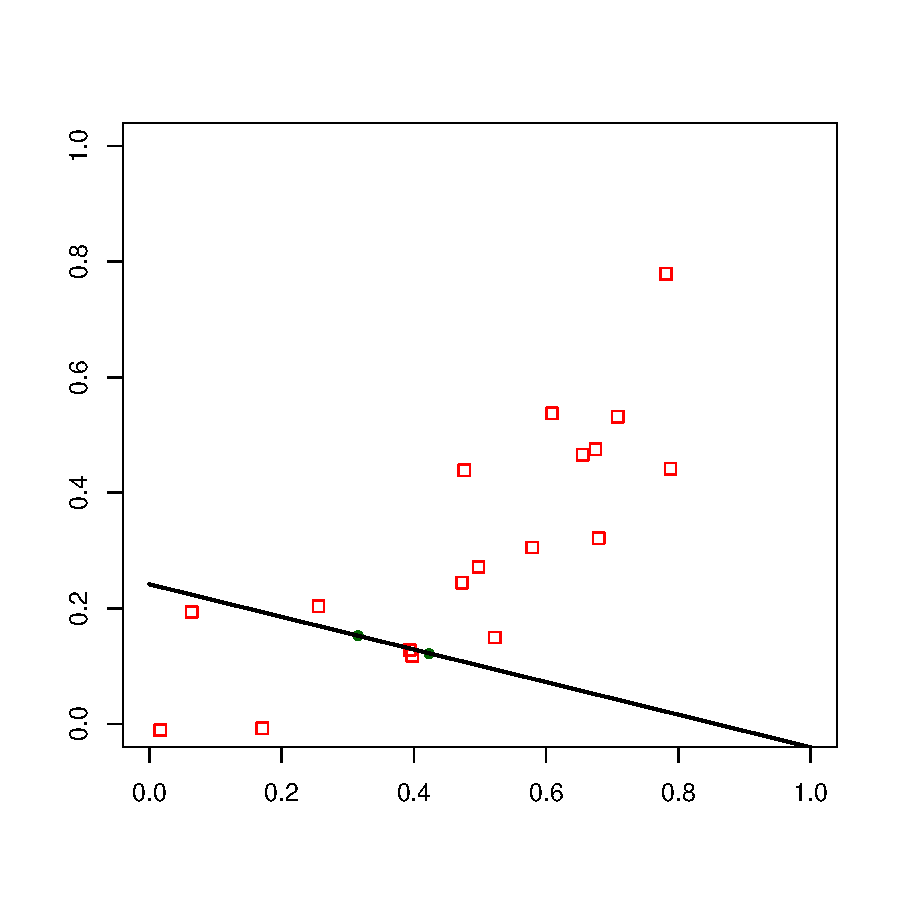
\includegraphics[width=10cm]{sample-split-1}\hspace*{1cm}
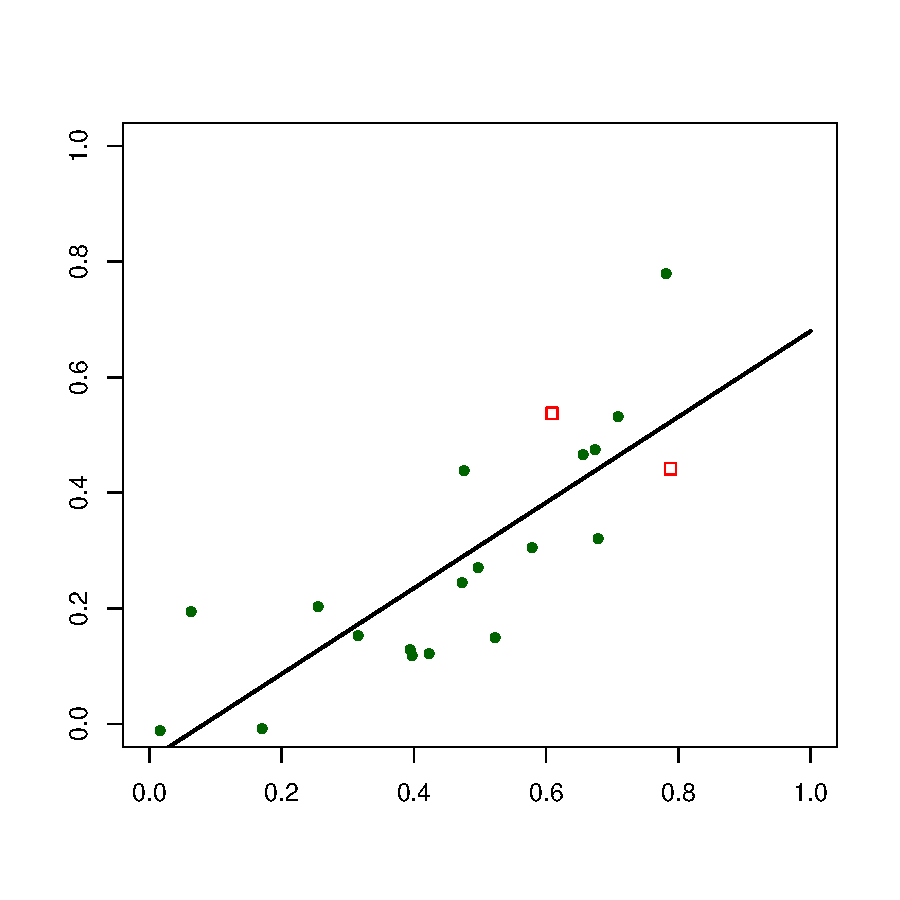
\includegraphics[width=10cm]{sample-split-2}
\end{center}
\vspace{-1cm}

If the number of available data points is small we have to choose:
\begin{triangles}
\item a small training set and bad model but good estimate on risk
\item a big training set and good model but bad estimate on risk
\end{triangles}

\foilhead[-1cm]{Why is holdout testing problematic}

\illustration[scale=0.8]{bias_variance_dilemma_1}
\vspace*{-.5cm}
Typical tradeoffs between learning-bias and variance of the validation error.   

\foilhead[-1.2cm]{Crossvalidation as an engineering trick}

\enlargethispage{0.7cm}

To reduce holdout error, we can do several holdout experiments. 
Since we do not have enough data, we redo splitting and training on the same data. 

This idea yields a generic crossvalidation scheme
\begin{enumerate}
\item Generate several splits of test and training data
\item For each split train the model and compute holdout error
\item Tabulate results\vspace*{2ex}
\begin{center}
\begin{tabular}{|l|c|c|c|c|}
\hline
 & Split $1$ & Split $2$ & $\ldots$ & Split $k$\\
 \hline
 Training error & $S_1$ & $S_2$ & $\ldots$ & $S_k$\\
 Test error     & $E_1$ & $E_2$ & $\ldots$ & $E_k$\\
\hline
 Optimism $\Delta$    & $E_1-S_1$ & $E_2-S_2$ & $\ldots$ & $E_k-S_k$\\
 \cline{2-5}
\hline
\end{tabular}
\end{center}
\vspace*{2ex}
\item Compute averages $E=\frac{1}{k}(E_1+\cdots+E_k)$ and $\Delta=\frac{1}{k}(\Delta_1+\cdots+\Delta_k)$
\item Visualise results and compute confidence intervals for estimates if needed. 
\end{enumerate}


\foilhead[-1cm]{What does crossvalidation measure?}

For each fold we have a separate predictor $f_i$ and test error $E_i$:
\begin{triangles}
\item Average $E$ characterises average behaviour of $f_1,\ldots, f_k$.
\item Algorithm can use only (1-1/k) fraction of the available data.
\item If there is not enough data for training $E$ overestimates the error. \vspace*{1cm}  
\end{triangles}

To estimate the performance of a classifier $f$ trained on the entire data:
\begin{triangles}
\item We must estimate the difference between test and training error $\Delta(f)$.
\item For normal ML algorithm optimism decreases by increasing the size $n$.
\item Crossvalidation estimates $\Delta$ at the point $(1-1/k)\cdot n \lesssim n$. 
\item Hence we can go from training error to test error estimate.
\item Training and test set fluctuations influence the outcome.  
\end{triangles}
 

\foilhead[-1cm]{Crossvalidation vs holdout estimates}

\illustration[scale=0.8]{crossvalidation_vs_holdout}
\vspace*{-.5cm}
\begin{triangles}
\item Crossvalidation error is slightly larger as the training set is smaller.  
\item Crossvalidation error is slightly more fluctuating due to correlations. 
\item Quite often these effects are quite small in practice. 
\end{triangles}



\foilhead[-1cm]{Theoretical explanation}

\textbf{Theorem.} 
Crossvalidation error $E =\frac{1}{k}(E_1+\cdots+E_k)$ is an 
unbiased estimate for the average test error that is taken over all models that are trained on $(1-1/k)\cdot n$ samples. 

\textbf{Proof}
\begin{align*}
\EXP[E] =\frac{\EXP[E_1]+\cdots+\EXP[E_k]}{k}=\EXP_{tr}\biggl[\EXP_{\vec{x}, y}\bigl[L(f(\vec{x}),y)|f=\AAA(train)\bigr]\biggr]
\end{align*}
where 
\begin{triangles}
\item the outer expectation is taken over all possible training sets  
\item the inner expectation measures the risk of the fitted model
\end{triangles}


\foilhead[-1cm]{Crossvalidation variance estimate}

\centerline{
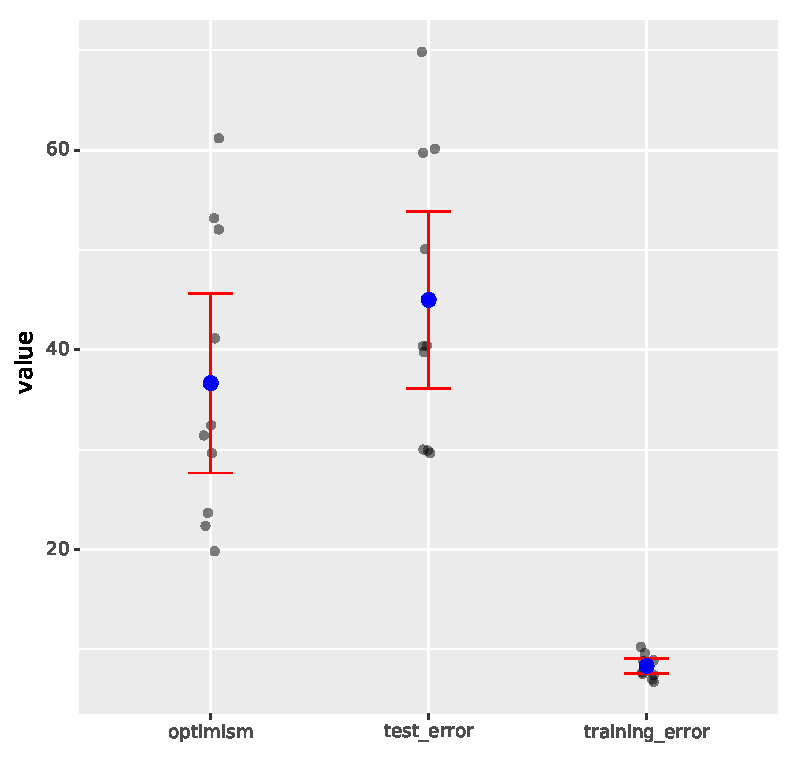
\includegraphics[scale=0.8]{crossvalidation_moment_matching}\hspace*{0.5cm}
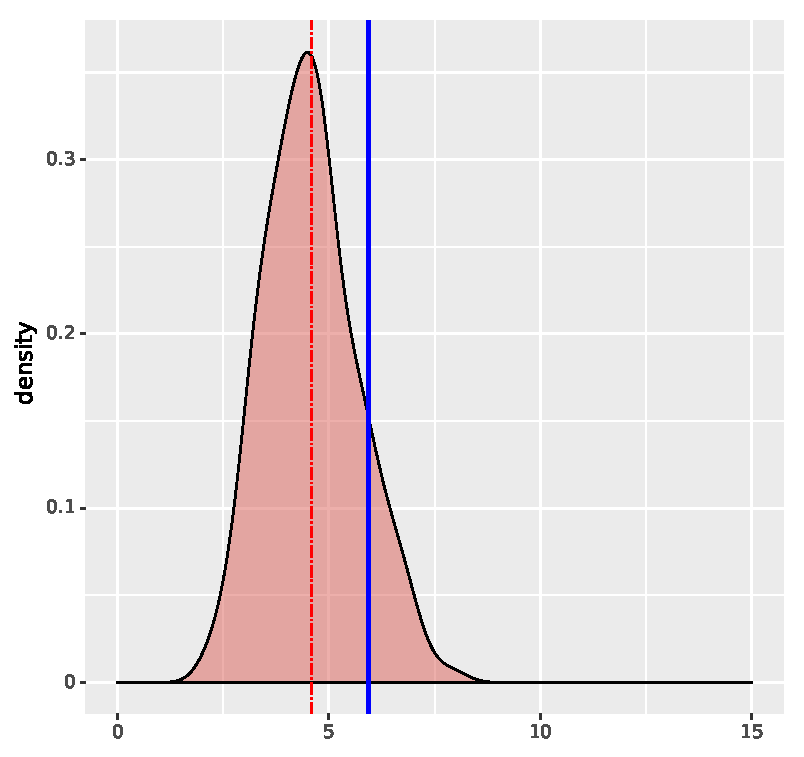
\includegraphics[scale=0.8]{crossvalidation_variance_estimate}}
\vspace*{-.5cm}
\begin{triangles}
\item The naive variance estimate for the crossvalidation error is biased.   
\item The estimate usually gives smaller confidence intervals as they are.  
\item This must be accounted in the estimates of optimism and test error. 
\end{triangles}



\foilhead[-1cm]{Theoretical explanation}

\textbf{Theorem.}
The variance of crossvalidation error $E =\frac{1}{k}(E_1+\cdots+E_k)$ is a weighted average consisting of three components
\begin{align*}
\theta = \frac{1}{n}\cdot\sigma^2+\textcolor{red}{\frac{m-1}{n} \cdot\omega + \frac{n-m}{n}\cdot\gamma}
\end{align*} 
where
\begin{triangles}
\item $m$ is the number of samples in each fold, i.e., $m\approx n/k$. 
\item $\sigma^2$ is the average variance of true test examples.
\item $\omega$ is the within-block covariance of test errors sharing the same test set. 
\item $\gamma$ is the between-block covariance of test errors cause by the fact that 
\begin{diamonds}
 \item training set have large intersection
 \item test fold is inside the training set of another split. 
\end{diamonds}   
\end{triangles}

 





\foilhead[-1cm]{What else can we do with crossvalidation?}

\textbf{Comparing different algorithms}
\begin{triangles}
\item We can tune hyperparameters of the algorithm
\item We can estimate which algorithm on average behaves better
\item We can quantify the stability of the performance ranking\vspace*{0.5cm}
\end{triangles} 

\textbf{Estimating variance of model parameters}
\begin{triangles}
\item Different folds give different parameter instances
\item Parameter confidence intervals can be used for diagnostics
\item Confidence intervals can be used for pruning spurious coefficients\vspace*{0.5cm}
\end{triangles} 

\textbf{Finding hard instances}
\begin{triangles}
\item Different folds give different mismatches $\hat{y}_i\neq y_i$
\item Corresponding problem instances $(\vec{x}_i, y_i)$ can be studied further
\end{triangles}


\foilhead[-1cm]{Estimating variance of model parameters}

\centerline{
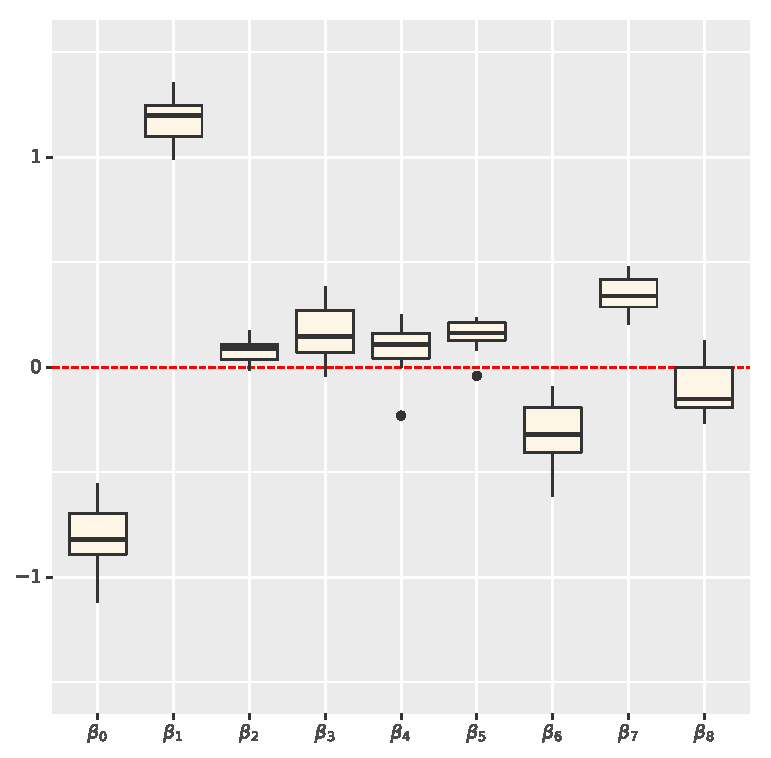
\includegraphics[scale=0.8]{crossvalidation_parameter_variance_i}\hspace*{0.5cm}
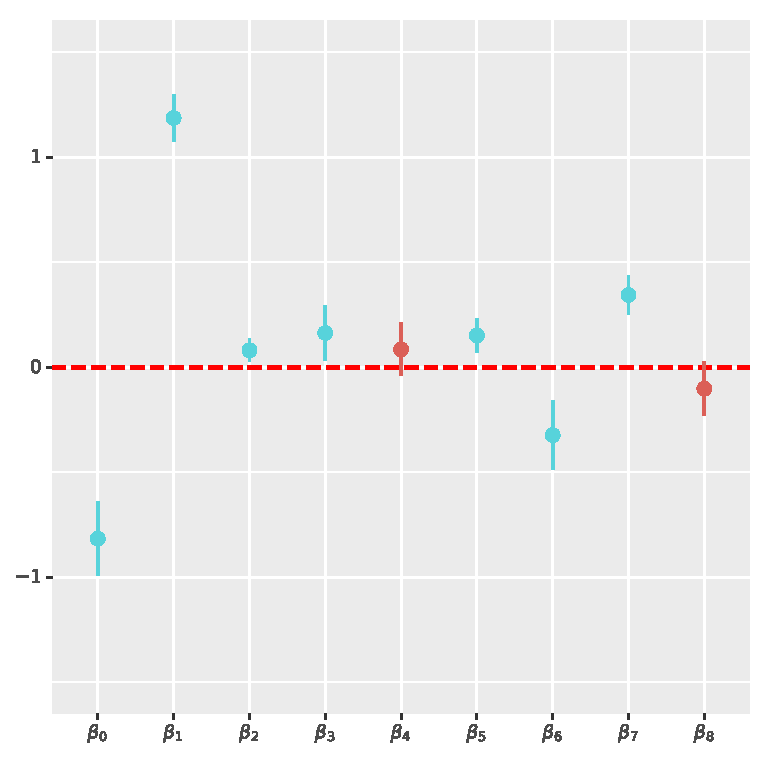
\includegraphics[scale=0.8]{crossvalidation_parameter_variance_ii}}
\vspace*{-.5cm}
\begin{triangles}
\item The method is applicable for models with compact parametrisation.
\item Each split defines a new model $f_i$ with coefficient $\vec{\beta}$.   
\item The variability of a coefficient $\beta_i$ shows its certainty and relevance. 
\end{triangles}


\foilhead[-1cm]{Other flavours of cross validation}

\textbf{Exhaustive data splitting}
\begin{triangles}
\item Leave-one-out method, leave-$p$-out method
\end{triangles}
\vspace*{1cm}

\textbf{Partial splitting}
\begin{triangles}
\item $K$-fold cross validation for $K = 5 , 10$ 
\item Monte-Carlo crossvalidation with a fixed split ratio, e.g $1:9$.\\ Same split can occur more than once  
\item Repeated learning testing with  a fixed split ratio, e.g $1:9$.
\\ Same split can occur only once. 
\end{triangles}


\foilhead[-1cm]{Bootstrapping as an alternative}

We could use the entire date set for validation if we could get another dataset for training the model. Bootstrapping is an engineering trick to create a new dataset out of a thin air.
\begin{enumerate}
\item Draw $N$ samples from the original dataset with replacement to get a \emph{bootstrap sample} $D_{B}$, e.g. the same element can occur more than once.
\item Train the model  on the bootstrap sample $D_B$.
\item Estimate the test error on the original dataset $D$.
\item Repeate the procedure $20$-$200$ times.
\item Compute necessary statistics and visualise the results if needed.
\end{enumerate}


\foilhead[-1cm]{Standard way how to use bootstrapping}
 
Bootstrapping is mostly used to estimate optimism
\begin{triangles}
\item The model is trained and the training error $S_i$ is computed.
\item The test error $E_i$ is usually computed on the entire dataset.
\item Optimism is computed as $E_i-S_i$.
\end{triangles}

\bigskip

Note that it does not make sense to compute test error on the entire dataset as we have used some of the data to build a model. Advanced bootstrap methods like \textbf{.632 bootstrap} and \textbf{.632 bootstrap+} use only the out of training set error and later find a tradeoff between training an test error.
\begin{align*}
E_{\text{boot}}=0.368\cdot S_{\text{Train}} + 0.632\cdot E_{\text{Out-of-training-set}}
\end{align*}

\foilhead[-1cm]{Other uses of bootstrapping}

Estimate the noise-tolerance of the machine learning method
\begin{triangles}
\item Generate a bootstrap sample.
\item Corrupt with an appropriate noise.
\item Train the model and estimate the performance.
\end{triangles}
\vspace*{2cm}

Estimate the variance of model coefficients
\begin{triangles}
\item Generate a bootstrap sample.
\item Estimate model parameters.
\item Visualise parameters and compute empirical quantiles.
\item Drop parameter which fluctuate around zero.
\end{triangles}


\end{document}